%
\section{Математическая модель}
%
В работе проводится моделирование трехфазной неизотермической фильтрации 
несмешивающихся жидкостей и газа с учетом их сжимаемости. Скелет породы
считаем неподвижным, пористость и плотность породы -- постоянными во всем
рассматриваемом объеме, среду -- изотропной, жидкие фазы -- слабосжимаемыми,
газ -- идеальным, температуру -- единой для всех фаз.

Рассматриваются одномерные, двумерные и трехмерные
области, заданные в декартовых координатах.

Рассмотрим более детально описанные в главе, посвященной физической
модели, законы и принципы с учетом введенных ограничений и опишем
используемые зависимости физических свойств фаз.

Пусть трехфазная система представляет собой две жидкие фазы -- вода и легкий
нефтяной продукт(LNAPL -- от английского Light Non-Aqueous Phase Liquids,
плотность меньше плотности воды), и одну газообразную.
Для удобства введем индексные обозначения для разных фаз: $w$ -- вода, $n$ --
легкая нефть, $g$ -- газ.

В качестве базовых переменных выбираем насыщенности, давления фаз и температуру.
Причем для насыщенностей в силу определения справедливо  $S_w + S_n + S_g = 1$.
А давления $P_n$ и $P_g$ отличаются от $P_w$ на величины капиллярных
давлений, являющихся функциями от насыщенностей.

Вводятся эффективные насыщенности каждой из фаз:
$\overline{S_i}={\dfrac{S_i-S_{ir}}{1-S_{wr}-S_{nr}-S_{gr}}}$, где , ${\quad}i=w,n,g$, $S_{wr}$,
$S_{nr}$, $S_{gr}$ -- остаточные насыщенности фаз.

Для описания
капиллярных давлений выбрана приближенная модель Паркера\cite{Parker}:
$$P_{cnw}(\overline{S_w})=P_n-P_w={\frac{1}{\gamma \delta_{nw}}}
\left( \overline{S_w}^{\frac{n}{1-n}}-1 \right)^\frac{1}{n},\;0<\overline{S_w}<1 $$
$$P_{cgn}(\overline{S_g})=P_g-P_n={\frac{1}{\gamma \delta_{gn}}}
\left( (1-\overline{S_g})^{\frac{n}{1-n}}-1 \right)^\frac{1}{n},\;0<\overline{S_g}<1$$
(где $P_{cnw}(\overline{S_w})$ - и $P_{cgn}(\overline{S_g})$- капиллярные давления на границах вода-нефть и нефть-газ, 
соответственно, $n$ и $\gamma $ -- пареметры породы Ван Генухтена из соответствующего приближения
Ван Генухтена\cite{Genuchten}, $\delta_{nw}$, $\delta_{gn}$ -- коэффициенты, определяемые поверхностным натяжением 
жидкостей). В работе используются следующие значения параметров: $n$ = 3.25, $\gamma $ = 0.00048Па$^{-1}$,
$\delta_{nw}$ = 0.67, $\delta_{gn}$ = 2. На участках, где эффективные насыщенности перестают удовлетворять
указанному интервалу, гладко продалжаем указанные функции капиллярных давлений. Изобразим полученные зависимости
на графиках:
\begin{center}
 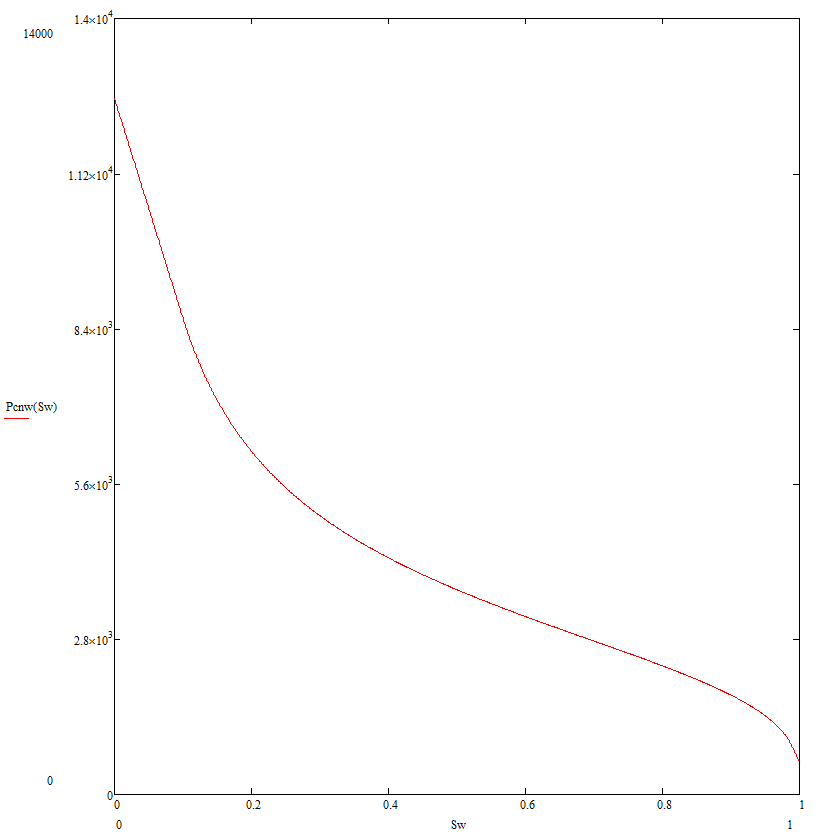
\includegraphics[width=7cm,height=9cm]{Pcnw}
 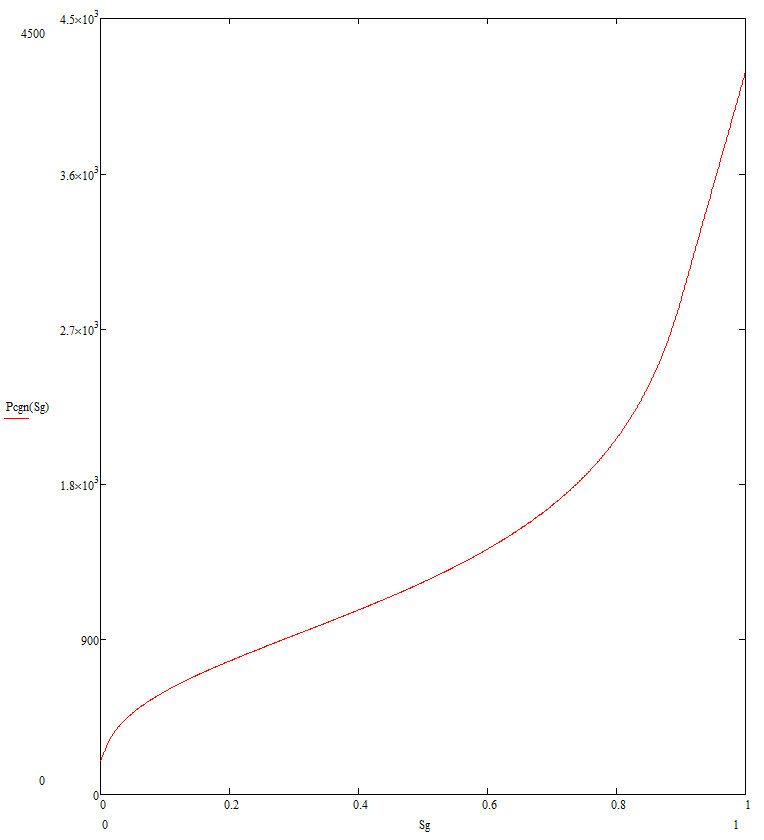
\includegraphics[width=7cm,height=9cm]{Pcgn}
\end{center}

Относительные фазовые проницаемости определяются в работе в соответствии с
приближением Стоуна в модификации Азиза и Сеттари\cite{Aziz-Settari}:

\begin{equation*}
  k_{w}(\overline{S_w})=
  \begin{cases}
  &\overline{S_w}^\frac{1}{2} \left( 1-\left( 1-\overline{S_w}^\frac{n}{n-1} \right) ^\frac{n-1}{n} \right) ^2
  \text{ , $0<\overline{S_w}<1$}\\
  &1 \text{ , $\overline{S_w}\ge 1$}\\
  &0 \text{ , $\overline{S_w}\le 0$}
\end{cases} 
\end{equation*}
\begin{equation*}
  k_{g}(\overline{S_g})=
  \begin{cases}
  &\overline{S_g}^\frac{1}{2} \left( 1-\left ( 1-\overline{S_g} \right) ^\frac{n}{n-1} \right) ^\frac{2(n-1)}{n}
  \text{ , $0<\overline{S_g}<1$}\\
  &1 \text{ , $\overline{S_g}\ge 1$}\\
  &0 \text{ , $\overline{S_g}\le 0$}
  \end{cases} 
\end{equation*}
\begin{center}
 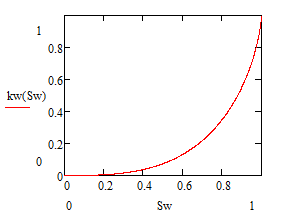
\includegraphics[width=7cm,height=6cm]{kw}
 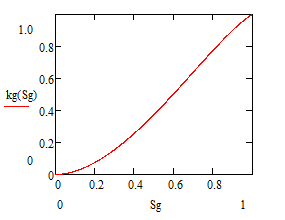
\includegraphics[width=7cm,height=6cm]{kg}
\end{center}
\begin{equation*}
  k_{n}(\overline{S_w},\overline{S_n})=
  \begin{cases}
  &\dfrac{\overline{S_n} k_{nw}(\overline{S_w})k_{ng}(\overline{S_n})}{(1-\overline{S_w})(\overline{S_w}+\overline{S_n})}
  \text{ , $\overline{S_w}<1, \quad \overline{S_w}+\overline{S_n} >0$}\\
  &0 \text{ , иначе}
  \end{cases}\text { , где}
\end{equation*}\\
\begin{equation*}
  k_{nw}(\overline{S_w})=
  \begin{cases}
  &(1-\overline{S_w})^\frac{1}{2} \left(1-\overline{S_w}^\frac{n}{n-1} \right) ^\frac{2(n-1)}{n}
  \text{ , $0<\overline{S_w}<1$}\\
  &1 \text{ , $\overline{S_w}\le 0$}\\
  &0 \text{ , $\overline{S_w}\ge 1$}
  \end{cases}\text { , }
\end{equation*}
\begin{equation*}
  k_{ng}(\overline{S_n})=
  \begin{cases}
  &\overline{S_n}^\frac{1}{2} \left( 1-\left( 1-\overline{S_n}^\frac{n}{n-1} \right) ^\frac{n-1}{n} \right) ^2 
  \text{ , $0<\overline{S_n}<1$}\\
  &1 \text{ , $\overline{S_n}\ge 1$}\\
  &0 \text{ ,  $\overline{S_n}\le 0$}
\end{cases}
\end{equation*}
\begin{center}
 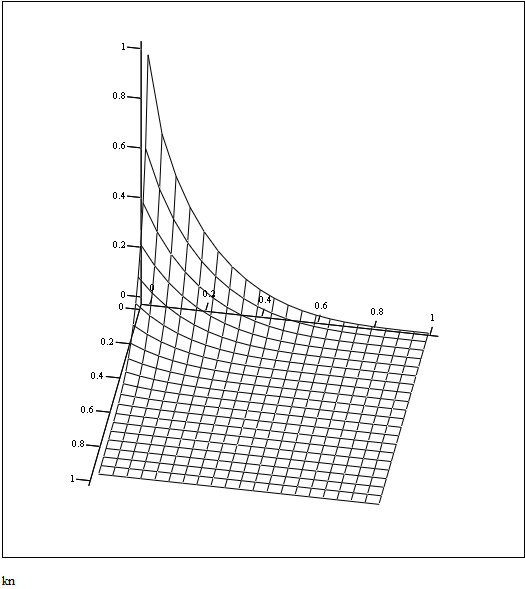
\includegraphics[width=12cm,height=12cm]{kn}
\end{center}
 
Таким образом, относительные проницаемости воды и газа являются функциями одной 
переменной(насыщенности одной из фаз), а нефти -- двух.

Используются следующие зависимости (собранные из различных справочников по физике)
для динамических вязкостей фаз:
\begin{equation}
  \begin{aligned}
    &\mu_w(T)=\frac{1}{29.21\times(T - 7506.64)},\\
    &\mu_n(T)=7.256\times10^{-10} \times e^{\frac{4141.9}{T}},\\
    &\mu_g(T)=1.717\times10^{-5} \times \left(\frac{T}{T_0}\right)^{0.683},
  \end{aligned}
\end{equation}
для коэффициентов теплопроводности:
\begin{equation}
  \begin{aligned}
    &\lambda_w(T)=0.553\times(1-0.003\times(T-T_0)),\\
    &\lambda_n(T)=0.14\times(1-0.001\times(T-T_0)),\\
    &\lambda_g(T)=0.237\times\left(\frac{T}{T_0}\right)^{0.82},\\
    &\lambda_r(T)=1.0,
  \end{aligned}
\end{equation}
для теплоемкостей при постоянном давлении:
\begin{equation}
  \begin{aligned}
    &C_{Pw}(T)= 4194 - 1.15 \times (T-T_0) + 0.015 \times (T-T_0)^2,\\
    &C_{Pn}(T)= 1700 - 3.4 \times (T-T_0),\\
    &C_{Pg}(T)= 1000 - 0.119 \times (T-T_0),\\
    &C_{Pr}(T)= 800 - 0.75 \times (T-T_0),
  \end{aligned}
\end{equation}
$T_0=273K$.

Перейдем к уравнениям состояний фаз.
Водную и нефтяную фазы считаем слабосжимаемыми и линейно зависящими от перепада температуры:\\
$${\rho}_i = {\rho}_{i0} {(1 + {\beta}_i (P_i-P_0) - {\alpha}_i (T-T_0))},
{\quad}0<{\beta}_{i}{\ll}1,{\quad}0<{\alpha}_{i}{\ll}1,{\quad}i=w,n,$$
где ${\rho}_{i0}$ -- известное значение плотности $i$-ой фазы, соответсвующее
значению давления $P_0$ и температуры $T_0$.

Для газа предполагаем справедливым уравнение состояния идеального
газа:
$${\rho}_g = {\rho}_{g0}{\frac{P_g}{P_0}}{\frac{T_0}{T}}.$$

В работе используются следующие значения:\\
$\rho_r=2000$ кг/м$^3$, $\rho_{w0}=1000$ кг/м$^3$,
$\rho_{n0}=850$ кг/м$^3$, $\rho_{g0}=1.4$ кг/м$^3$,\\
$\beta_w=4.4\cdot10^{-7}$ 1/Па, $\beta_n=10^{-6}$ 1/Па,
$\alpha_w=1.32\cdot10^{-7}$ 1/К, $\alpha_n=9.2\cdot10^{-7}$ 1/К.

Таким образом, полная система уравнений для описания трехфазной системы
принимает вид:
\begin{equation}
\left\{
  \begin{aligned}
    &\frac{\partial \left(m {\sum\limits_{i}{\rho_i S_i E_i(P_i, T)}} + (1-m){\rho_r E_r(P_w, T)}\right)}{\partial t}
      + div(\sum_{i}{\rho_i H_i(T) \overrightarrow{u_i}}) = div(\lambda_{eff} grad T) \\
    &\frac{\partial (m \rho_i S_i)}{\partial t}+ div(\rho_i \overrightarrow{u_i}) = \rho_i q_i \\
    &\overrightarrow{u_i}=-K \frac{k_i}{{\mu_i(T)}}(grad P_i - {\rho}_i\overrightarrow{g})\\
    &i=w,n,g\\
    &P_n=P_w+P_{cnw}(\overline{S_w})\\
    &P_g=P_w+P_{cnw}(\overline{S_w})+P_{cgn}(\overline{S_g})\\
    &S_w + S_n + S_g=1\\
    &k_w=k_w(\overline{S_w}),\quad k_g=k_g(\overline{S_g}),\quad k_n=k_n(\overline{S_w},\overline{S_n})\\
    &\rho_i=\rho_i(P_i,T)
  \end{aligned}
\right.
\end{equation}

Где $\rho_i q_i$ -- источниковые члены, индекс $r$ обозначает твердую породу.
Используемые параметры породы: $K=6.64\cdot 10^{-11}$ м$^2$, $m$=0.4.
Все значения констант приводятся в системе единиц СИ.

В зависимости от конкретной постановки задачи в работе используются различные
граничные условия. На границе поддерживается постоянное давление, или же оно
определяется из условия непротекания фазы (нормальная компонента скорости
фазы на границе равна 0, $\overrightarrow{u_i}_{n} = 0$).
Для насыщенности ставится условие равенства нулю потока через граничную 
поверхность или же задается поток насыщенности в виде известной функции через 
$ \dfrac{\partial S_i}{\partial n}, \; i=w,n, \;  n \text{-- нормаль к границе} $.
Также для насыщенности может быть задано некоторое постоянное значение на границе.
Для температуры тоже ставятся граничные условия первого или второго рода. 

В начальный момент времени считаем известными распределения давления водной 
фазы, насыщенностей фаз и температуры по всей области.
